\documentclass[12pt]{article}


\usepackage[english]{babel}
\usepackage[utf8]{inputenc}
\usepackage{amsmath,amssymb}
\usepackage{listings} % untuk kode python
\usepackage{xcolor}

\definecolor{codegreen}{rgb}{0,0.6,0}
\definecolor{codegray}{rgb}{0.5,0.5,0.5}
\definecolor{codepurple}{rgb}{0.58,0,0.82}
\definecolor{backcolour}{rgb}{0.95,0.95,0.92}

\lstdefinestyle{mystyle}{
    backgroundcolor=\color{backcolour},   
    commentstyle=\color{codegreen},
    keywordstyle=\color{magenta},
    numberstyle=\tiny\color{codegray},
    stringstyle=\color{codepurple},
    basicstyle=\ttfamily\footnotesize,
    breakatwhitespace=false,         
    breaklines=true,                 
    captionpos=b,                    
    keepspaces=true,                 
    numbers=left,                    
    numbersep=5pt,                  
    showspaces=false,                
    showstringspaces=false,
    showtabs=false,                  
    tabsize=2
}

\lstset{style=mystyle}
%\usepackage{parskip}
\usepackage{graphicx}

% Margins
\usepackage[top=2.5cm, left=3cm, right=3cm, bottom=4.0cm]{geometry}
\usepackage{hyperref}
\usepackage{natbib}
\usepackage{comment}
\setlength\bibsep{1em}
\setlength\bibhang{1.5em}
\renewcommand\bibfont{\singlespace}
\bibliographystyle{dcu}
% Colour table cells
%\usepackage[table]{xcolor}

% Get larger line spacing in table
\newcommand{\tablespace}{\\[1.25mm]}
\newcommand\Tstrut{\rule{0pt}{2.6ex}}         % = `top' strut
\newcommand\tstrut{\rule{0pt}{2.0ex}}         % = `top' strut
\newcommand\Bstrut{\rule[-0.9ex]{0pt}{0pt}}   % = `bottom' strut

%%%%%%%%%%%%%%%%%
%     Title     %
%%%%%%%%%%%%%%%%%
\title{Exercise 5 - Regularized Linear Regression and Bias v.s. Variance}
\author{Azka NA}
\date{\today}

\begin{document}
\maketitle

%%%%%%%%%%%%%%%%%
%   Problem 1   %
%%%%%%%%%%%%%%%%%

\section{Introduction}
This is the guide for Andrew Ng's Machine Learning course programming assignment done in Python, adapted from the original guide written for Octave or MATLAB.

In this exercise, you will implement regularized linear regression and use it to study models with different bias-variance properties. Before starting on this programming exercise, we strongly recommend watching the video lectures and completing the review questions for the associated topics

For Programming Exercise 5: Regularized Linear Regression and Bias v.s. Variance, you will need to download the following files:

\texttt{exercise5.ipynb} - Jupyter notebook containing the script

\texttt{ex5data1.mat} - Dataset

\hrulefill

\section{Regularized Linear Regression}

In the first half of the exercise, you will implement regularized linear regression to predict the amount of water flowing out of a dam using the change of water level in a reservoir. In the next half, you will go through some diagnostics of debugging learning algorithms and examine the effects of bias v.s. variance.

\subsection{Visualizing the dataset}

We will begin by visualizing the dataset containing historical records on the change in the water level, $x$, and the amount of water flowing out of the dam, $y$, as shown in Figure~\ref{fig:scatter}

This dataset is divided into three parts:

\begin{itemize}
  \item A \textbf{training} set that your model will learn on: \texttt{X, y}
  \item A \textbf{cross validation} set for determining the regularization parameter: \texttt{Xval, yval}
  \item A \textbf{test} set for evaluating performance. These are "unseen" examples which your model did not see during training: \texttt{Xtest, ytest}
\end{itemize}

In the following parts, you will implement linear regression and use that to fit a straight line to the data and plot learning curves. Following that, you will implement polynomial regression to find a better fit to the data.

\begin{figure}[h!]
  \centering
  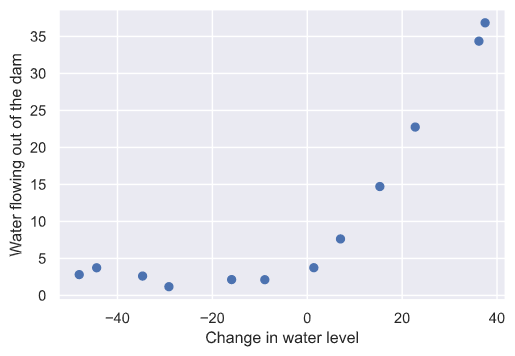
\includegraphics[scale=0.6]{scatter.png}
  \caption{Data}
  \label{fig:scatter}
\end{figure}

\subsection{Regularized linear regression cost function}
Recall that regularized linear regression has the following cost function:

\begin{align}
  J(\theta_1) & = \frac{1}{2m}\Big(\sum_{i=1}^m{(h_\theta(x^{(i)})-y^{(i)})^2}\Big) + \frac{\lambda}{2m}\Big(\sum_{j=1}^n{{\theta_j}^2}\Big),
\end{align}

where $\lambda$ is a regularization parameter which controls the degree of regularization (thus, help preventing overfitting). The regularization term puts a penalty on the overall cost $J$. As the magnitudes of the model parameters $\theta_j$ increase, the penalty increases as well. Note that you should not regularize the $\theta_0$ term.

Your task is to write a function to calculate the regularized linear regression cost function. If possible, try to vectorize your code and avoid writing loops.

\begin{lstlisting}[language=Python]
  def linearRegCostFunction(X, y, theta, Lambda):
    m = len(y)
    y = y.reshape(m,1)
    grad = np.zeros(theta.shape)
    n_1 = theta.shape[0]
    theta = theta.reshape(n_1,1)
    cost = 0
    h = np.dot(X, theta)
    cost = 1/(2*m) * np.sum((h-y)**2)
    cost_reg = cost + Lambda/(2*m)*np.sum(theta[1:]**2)

    grad[0] = (1/m)*(X[:,0:1].reshape(m,1)*(h - y)).sum(axis=0)
    grad[1:] = (1/m)*( (X[:,1:]*(h - y)).sum(axis=0)  + Lambda*theta[1:].reshape(n_1-1))

    return cost_reg, grad
\end{lstlisting}

When you are finished, run your cost function using \texttt{theta} initialized at \texttt{[1,1]}. You should expect to see an output of 303.993.

\subsection{Regularized linear regression gradient}

Correspondingly, the partial derivative of regularized linear regression's cost for $\theta_j$ is defined as

\begin{align}
  \frac{\partial J(\theta)}{\partial \theta_0} & = \frac{1}{m}\sum_{i=1}^m{(h_\theta(x^{(i)})-y^{(i)}) x_j^{(i)}} & \text{for} j & = 0 \\
  \frac{\partial J(\theta)}{\partial \theta_j} & = \bigg(\frac{1}{m}\sum_{i=1}^m{(h_\theta(x^{(i)})-y^{(i)}) x_j^{(i)}}\bigg) + \frac{\lambda}{m}\theta_j & \text{for} j & \geq 1
\end{align}


Run your cost function using theta initialized at [1,1]. You should expect to see a gradient of \texttt{[-15.30, 598.250]}.

\subsection{Fitting linear regression}

Once your cost function and gradient are working correctly, compute the optimal values of $\theta$ using the \texttt{minimize} function from Scipy's \texttt{Optimize} module.

In this part, we set regularization parameter $\lambda$ to zero. Because our current implementation of linear regression is trying to fit a 2-dimensional $\theta$, regularization will not be incredibly helpful for a $\theta$ of such low dimension. In the later parts of the exercise, you will be using polynomial regression with regularization.

\begin{lstlisting}[language=Python]
  def trainLinearReg(linearRegCostFunction, X, y, Lambda=0, maxiter=200):

    initial_theta = np.zeros(X.shape[1])
    costFunction = lambda t: linearRegCostFunction(X, y, t, Lambda)
    options = {'maxiter': maxiter}
    minimizef = optimize.minimize(costFunction, initial_theta, jac=True, method='TNC', options=options)
    return minimizef.x 
\end{lstlisting}

Finally, we should also plot the best fit line, resulting in an image similar to Figure ~\ref{fig:linearfit}. The best fit line tells us that the model is not a good fit to the data because the data has a non-linear pattern. While visualizing the best fit as shown is one possible way to debug your learning algorithm, it is not always easy to visualize the data and model. In the next section, you will implement a function to generate learning curves that can help you debug your learning algorithm even if it is not easy to visualize the data.

\begin{figure}[h!]
  \centering
  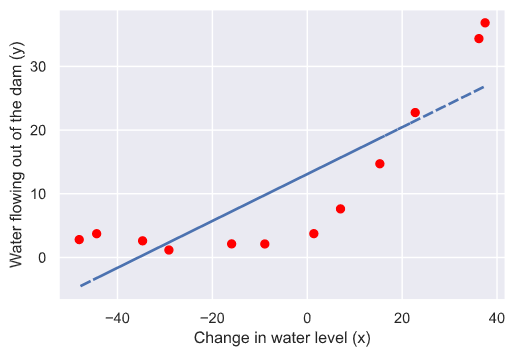
\includegraphics[scale=0.6]{linearfit.png}
  \caption{Linear fit}
  \label{fig:linearfit}
\end{figure}

\section{Bias-variance}

An important concept in machine learning is the bias-variance tradeoff. Models with high bias are not complex enough for the data and tend to underfit, while models with high variance overfit to the training data.

In this part of the exercise, you will plot training and test errors on a learning curve to diagnose bias-variance problems.

\subsection{Learning curves}

You will now implement code to generate the learning curves that will be useful in debugging learning algorithms. Recall that a learning curve plots training and cross-validation error as a function of training set size. Your job is to write a function so that it returns a vector of errors for the training set and cross-validation set.

To plot the learning curve, we need a training and cross-validation set error for different training set sizes. To obtain different training set sizes, you should use different subsets of the original training set \texttt{X}. Specifically, for a training set size of i, you should use the first i examples (i.e., \texttt{X[:i,:]} and \texttt{y[:i]}).

You can use the \texttt{trainLinearReg} function to find the $\theta$ parameters. Note that the lambda is passed as a parameter to the \texttt{learningCurve} function. After learning the $\theta$ parameters, you should compute the \textbf{error} on the training and cross-validation sets. Recall that the training error for a dataset is defined as

\begin{align}
  J(\theta_1) & = \frac{1}{2m}\bigg[\sum_{i=1}^m{(h_\theta(x^{(i)})-y^{(i)})^2}\bigg].
\end{align}

In particular, note that the training error does not include the regularization term. One way to compute the training error is to use your existing cost function and set $\lambda$ to 0 only when using it to compute the training error and cross-validation error. When you are computing the training set error, make sure you compute it on the training subset (i.e., \texttt{X[:n]} and \texttt{y[:n]}) (instead of the entire training set). However, for the cross-validation error, you should compute it over the entire cross-validation set. You should store the computed errors in the vectors \texttt{training\_error} and \texttt{validation\_error}.

\begin{lstlisting}[language=Python]
  def learningCurve(X, y, Xval, yval, Lambda=0):
    m = len(y)
    training_error = np.zeros(m)
    validation_error = np.zeros(m)

    for i in range(m):
        theta_optimized1 = trainLinearReg(linearRegCostFunction, X[:i+1], y[:i+1], Lambda)
        training_error[i], _ = linearRegCostFunction(X[:i+1], y[:i+1], theta_optimized1, Lambda)
        validation_error[i], _ = linearRegCostFunction(Xval, yval, theta_optimized1, Lambda)

    return training_error, validation_error
\end{lstlisting}

When you are finished, print the learning curves and make a plot similar to Figure~\ref{fig:learningcurve}.

\begin{figure}[h!]
  \centering
  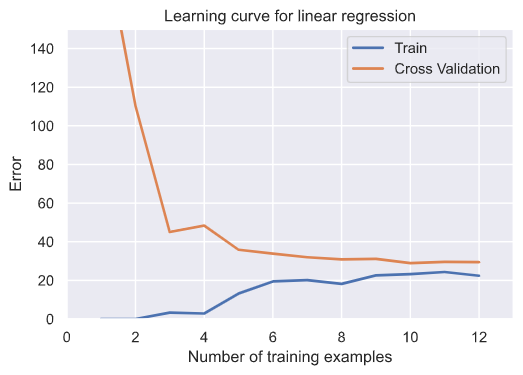
\includegraphics[scale=0.6]{learningcurve.png}
  \caption{Linear regression learning curve}
  \label{fig:learningcurve}
\end{figure}

In Figure~\ref{fig:learningcurve}, you can observe that both the train error and cross-validation error are high when the number of training examples is increased. This reflects a \textbf{high bias} problem in the model --- the linear regression model is too simple and is unable to fit our dataset well. In the next section, you will implement polynomial regression to fit a better model for this dataset.

\section{Polynomial regression}

The problem with our linear model was that it was too simple for the data and resulted in underfitting (high bias). In this part of the exercise, you will address this problem by adding more features.

For use polynomial regression, our hypothesis has the form:

\begin{align}
  h_\theta(x) & = \theta_0 + \theta_1 * (\text{waterLevel}) + \theta_2 * (\text{waterLevel})^2 + \dots + \theta_p * (\text{waterLevel})^p \\
   & = \theta_0 + \theta_1 x_1 + \theta_2 x_2 + \dots + \theta_p x_p 
\end{align}

Notice that by defining $x_1 = \text{(waterLevel)}$, $x_2 = \text{(waterLevel)}^2$, $\dots$, $x_p = \text{(waterLevel)}^p$, we obtain a linear regression model where the features are the various powers of the original value (waterLevel).

Now, you will add more features using the higher powers of the existing feature $x$ in the dataset. Your task in this part is to complete the code for \texttt{polyFeatures} so that the function maps the original training set \texttt{X} of size $m \times 1$ into its higher powers. Specifically, when a training set \texttt{X} of size $m \times 1$ is passed into the function, the function should return a $m \times p$ matrix \texttt{X\_poly}, where column 1 holds the original values of \texttt{X}, column 2 holds the values of $\verb!X.^2!$, column 3 holds the values of $\verb!X.^3!$, and so on. Note that you don’t have to account for the zero-eth power in this function.

\begin{lstlisting}[language=Python]
  def polyFeatures(X, p):
    m = X.shape[0]
    X_out = np.zeros((m,p))
    for i in range(p):
        X_out[:,i] = X.flatten()**(i+1)
    return X_out
\end{lstlisting}


Now you have a function that will map features to a higher dimension, then apply it to the training set, the test set, and the cross-validation set (which you haven’t used yet).

\subsection{Learning Polynomial Regression}

After you have completed \texttt{polyFeatures}, we will proceed to train polynomial regression using your linear regression cost function.

Keep in mind that even though we have polynomial terms in our feature vector, we are still solving a linear regression optimization problem. The polynomial terms have simply turned into features that we can use for linear regression. We are using the same cost function and gradient that you wrote for the earlier part of this exercise.

For this part of the exercise, you will be using a polynomial of degree 8. It turns out that if we run the training directly on the projected data, will not work well as the features would be badly scaled (e.g., an example with $x = 40$ will now have a feature $x_8 = 40^8 = 6.5 \times 10^{12}$). Therefore, you will need to use feature normalization.

Before learning the parameters $\theta$ for the polynomial regression, we will first call \texttt{featureNormalize} and normalize the features of the training set, storing the mu, sigma parameters separately. 

After learning the parameters $\theta$, you should see two plots (Figure~\ref{fig:polynomialfit},\ref{fig:polylearningcurve}) generated for polynomial regression with $\lambda = 0$.

\begin{figure}[h!]
  \centering
  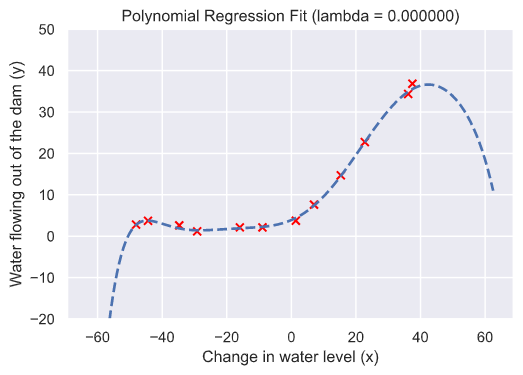
\includegraphics[scale=0.6]{polynomialfit.png}
  \caption{Polynomial fit, $\lambda = 0$}
  \label{fig:polynomialfit}
\end{figure}

\begin{figure}[h!]
  \centering
  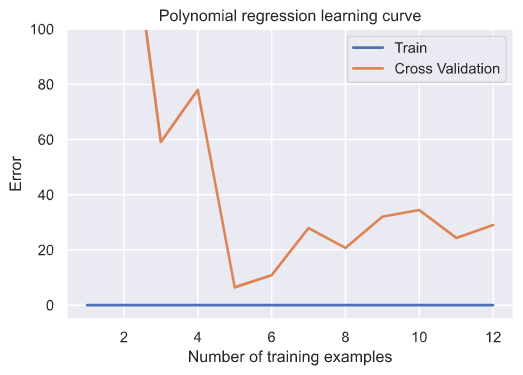
\includegraphics[scale=0.6]{polylearningcurve.png}
  \caption{Polynomial learning curve, $\lambda = 0$}
  \label{fig:polylearningcurve}
\end{figure}

From Figure ~\ref{fig:polynomialfit}, you should see that the polynomial fit is able to follow the datapoints very well - thus, obtaining a low training error. However, the polynomial fit is very complex and even drops off at the extremes. This is an indicator that the polynomial regression model is overfitting the training data and will not generalize well.

To better understand the problems with the unregularized ($\lambda = 0$) model, you can see that the learning curve (Figure~\ref{fig:polylearningcurve}) shows the same effect where the low training error is low, but the cross validation error is high. There
is a gap between the training and cross validation errors, indicating a high
variance problem.

One way to combat the overfitting (high-variance) problem is to add regularization to the model. In the next section, you will get to try different $\lambda$ parameters to see how regularization can lead to a better model.

\subsection{Optional (ungraded) exercise: Adjusting the regularization parameter}

In this section, you will get to observe how the regularization parameter affects the bias-variance of regularized polynomial regression. You should now modify the the \texttt{Lambda} parameter and try $\lambda = 1, 100$. For each of these values, the script should generate a polynomial fit to the data and also a learning curve.

For $\lambda = 1$, you should see a polynomial fit that follows the data trend well (Figure~\ref{fig:polyfit1}) and a learning curve (Figure~\ref{fig:polycurve1}) showing that both the cross-validation and training error converge to a relatively low value. This shows the $\lambda = 1$ regularized polynomial regression model does not have the highbias or high-variance problems. In effect, it achieves a good trade-off between bias and variance.

For $\lambda = 100$, you should see a polynomial fit (Figure~\ref{fig:polyfit100}) that does not follow the data well. In this case, there is too much regularization and the model is unable to fit the training data.

\begin{figure}[h!]
  \centering
  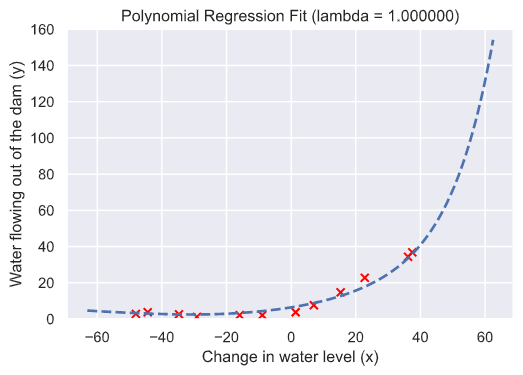
\includegraphics[scale=0.6]{polyfit1.png}
  \caption{Polynomial fit, $\lambda = 1$}
  \label{fig:polyfit1}
\end{figure}

\begin{figure}[h!]
  \centering
  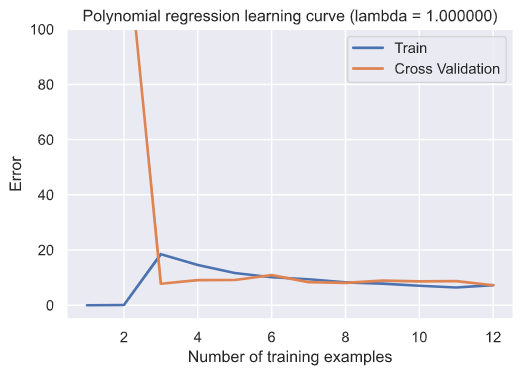
\includegraphics[scale=0.6]{polycurve1.png}
  \caption{Polynomial learning curve, $\lambda = 1$}
  \label{fig:polycurve1}
\end{figure}

\begin{figure}[h!]
  \centering
  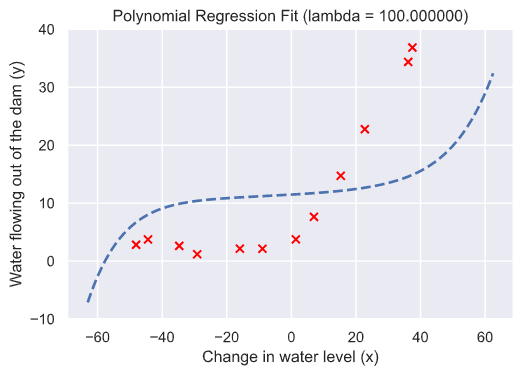
\includegraphics[scale=0.6]{polyfit100.png}
  \caption{Polynomial fit, $\lambda = 100$}
  \label{fig:polyfit100}
\end{figure}

\subsection{Selecting $\lambda$ using a cross validation set}

From the previous parts of the exercise, you observed that the value of $\lambda$ can significantly affect the results of regularized polynomial regression on the training and cross-validation set. In particular, a model without regularization ($\lambda = 0$) fits the training set well, but does not generalize. Conversely, a model with too much regularization ($\lambda = 100$) does not fit the training set and testing set well. A good choice of $\lambda$ (e.g., $\lambda = 1$) can provide a good fit to the data.

In this section, you will implement an automated method to select the $\lambda$ parameter. Concretely, you will use a cross-validation set to evaluate how good each $\lambda$ value is. After selecting the best $\lambda$ value using the cross-validation set, we can then evaluate the model on the test set to estimate how well the model will perform on actual unseen data.

Your task is to complete the code for \texttt{validationCurve}. Specifically, you should should use the \texttt{trainLinearReg} function to train the model using different values of $\lambda$ and compute the training error and cross-validation error. You should try $\lambda$ in the following range: \{0, 0.001, 0.003, 0.01, 0.03, 0.1, 0.3, 1, 3, 10\}.

\begin{lstlisting}[language=Python]
  def validationCurve(X, y, Xval, yval):
    
    lambda_vec = [0, 0.001, 0.003, 0.01, 0.03, 0.1, 0.3, 1, 3, 10]

    training_error = np.zeros(len(lambda_vec))
    validation_error = np.zeros(len(lambda_vec))

    for i in range(len(lambda_vec)):
      lambda_try = lambda_vec[i]
      theta_t = trainLinearReg(linearRegCostFunction, X, y, Lambda = lambda_try)
      training_error[i], _ = linearRegCostFunction(X, y, theta_t, Lambda = 0)
      validation_error[i], _ = linearRegCostFunction(Xval, yval, theta_t, Lambda = 0)

    return lambda_vec, training_error, validation_error
\end{lstlisting}

\begin{figure}[h!]
  \centering
  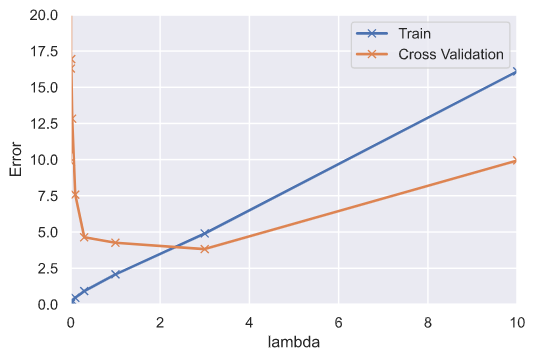
\includegraphics[scale=0.6]{selectlambda.png}
  \caption{Selecting $\lambda$ using a cross-validation set}
  \label{fig:selectlambda}
\end{figure}

After you have completed the code, run your function to plot a cross-validation curve of error v.s. $\lambda$ that allows you select which $\lambda$ parameter to use. You should see a plot similar to Figure ~\ref{fig:selectlambda}. In this figure, we can see that the best value of $\lambda$ is around 3. Due to randomness in the training and validation splits of the dataset, the cross-validation error can sometimes be lower than the training error.

\subsection{Optional (ungraded) exercise: Computing test set error}

In the previous part of the exercise, you implemented code to compute the cross-validation error for various values of the regularization parameter $\lambda$. However, to get a better indication of the model’s performance in the real world, it is important to evaluate the "final" model on a test set that was not used in any part of training (that is, it was neither used to select the $\lambda$ parameters, nor to learn the model parameters $\theta$).

For this optional (ungraded) exercise, you should compute the test error
using the best value of $\lambda$ you found. In our cross validation, we obtained a
test error of 3.8599 for $\lambda= 3$ .

\subsection{Optional (ungraded) exercise: Plotting learning curves with randomly selected examples}

In practice, especially for small training sets, when you plot learning curves to debug your algorithms, it is often helpful to average across multiple sets of randomly selected examples to determine the training error and cross validation error.

Concretely, to determine the training error and cross validation error for $i$ examples, you should first randomly select $i$ examples from the training set and $i$ examples from the cross validation set. You will then learn the parameters $\theta$ using the randomly chosen training set and evaluate the parameters $\theta$ on the randomly chosen training set and cross validation set. The above steps should then be repeated multiple times (say 50) and the averaged error should be used to determine the training error and cross validation error for $i$ examples.


\end{document}
